\begin{enunciado}
 Si se selecciona al azar una lata que contiene $500$ nueces de cada uno de tres diferentes distribuidores de nueces surtidas y contienen, respectivamente, $345$, $313$ y $359$ cacahuates en cada una de las latas, ¿con un nivel de significancia de $0.01$ podemos concluir que las nueces surtidas de los tres distribuidores contienen proporciones iguales de cacahuates?
\end{enunciado}

\begin{solucion}
 El problema corresponde a un ajuste de bondad a una distribuci\'on
 uniforme discreta. As\'{\i} pues, si se nombra $X$ a la distribuci\'on
 de cacahuates de los diferentes distribuidores en la lata de nueces
 surtidas, la hip\'otesis de prueba se escribe como sigue:
 \begin{eqnarray*}
  H_0: & & X \text{ sigue una distribuci\'on uniforme discreta } f(x;3) \\
  H_1: & & X\text{ no sigue una distribuci\'on uniforme discreta } f(x;3)
 \end{eqnarray*}
 donde $x \in \mathbb{N}\cap[1,3]$,
 con un nivel de significancia de $0.01$.
 \par 
 El proceso se puede realizar usando el programa de R escrito
 en el archivo adjunto con el nombre
 \texttt{P15\_Prueba\_de\_bondad\_chi2\_01.r},
 que a su vez usa el archivo \texttt{DB39\_Problema\_107.csv},
 con los siguientes cambios:
 \begin{verbatim}
> datos<-read.csv("DB39_Problema_107.csv",sep=";",encoding="UTF-8")
> varInteres<-"Frecuencia"
> varCelda<-"Cacahuates.cantidad"
> distribucion<-1
> parametro_nombre<-NULL
> parametro_valor<-NULL
> combinar<-TRUE
> grafica<-TRUE
> tituloEjeX<-"Cacahuates distintos en la lata de nueces surtidas"
> alfa<-0.01
 \end{verbatim}
 \vspace{-0.5cm}
 el programa de R lanza el siguiente resultado:
 \begin{verbatim}
             Variable Distribución de ajuste Estadístico Chisq2
1 Cacahuates.cantidad               Uniforme           3.280236
  Grados de libertad   Valor-p alpha Región de Rechazo
1                  2 0.1939572  0.01       > 9.2103404
                          Resultado
1 No se rechaza el ajuste de bondad
 \end{verbatim}
 \vspace{-0.5cm}
 que incluye la siguiente figura:
 \begin{center}
  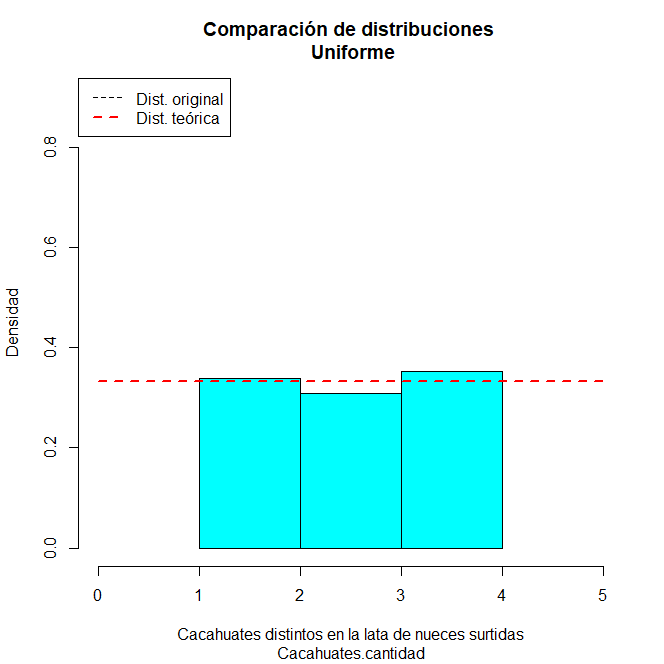
\includegraphics[scale=0.35]{Problema_107.png}
 \end{center}
 el cual incluyen la regi\'on de rechazo $\chi^2 > 9.2103404$,
 donde $\chi^2 = \sum_{i=0}^{k-1} \frac{\left( o_i - e_i \right)^2}{e_i}$,
 que se distribuye como una $\chi^2$ con $v=2$ grados de libertad,
 y el valor calculado del estad\'{\i}stico $\chi^2 = 3.280236$,
 junto con la decisi\'on que es clara, que indica que no hay evidencia
 para rechaza la hip\'otesis nula; adem\'as, el programa brinda m\'as
 informaci\'on como el valor $P$, que es igual a $0.1939572$.
 Por lo tanto, se considera que $X$ se ajusta bien a una distribuci\'on
 uniforme; es decir, con un nivel de significancia de $0.01$, se puede
 concluir que las nueces surtidas de los tres distribuidores
 contienen proporciones iguales de cacahuates.
 que es a lo que se quer\'{\i}a llegar.${}_{\blacksquare}$
\end{solucion}
